\documentclass[12pt,english,dvipsnames,aspectratio=169,handout]{beamer}\usepackage[]{graphicx}\usepackage[]{xcolor}
% maxwidth is the original width if it is less than linewidth
% otherwise use linewidth (to make sure the graphics do not exceed the margin)
\makeatletter
\def\maxwidth{ %
  \ifdim\Gin@nat@width>\linewidth
    \linewidth
  \else
    \Gin@nat@width
  \fi
}
\makeatother

\definecolor{fgcolor}{rgb}{0.345, 0.345, 0.345}
\newcommand{\hlnum}[1]{\textcolor[rgb]{0.686,0.059,0.569}{#1}}%
\newcommand{\hlstr}[1]{\textcolor[rgb]{0.192,0.494,0.8}{#1}}%
\newcommand{\hlcom}[1]{\textcolor[rgb]{0.678,0.584,0.686}{\textit{#1}}}%
\newcommand{\hlopt}[1]{\textcolor[rgb]{0,0,0}{#1}}%
\newcommand{\hlstd}[1]{\textcolor[rgb]{0.345,0.345,0.345}{#1}}%
\newcommand{\hlkwa}[1]{\textcolor[rgb]{0.161,0.373,0.58}{\textbf{#1}}}%
\newcommand{\hlkwb}[1]{\textcolor[rgb]{0.69,0.353,0.396}{#1}}%
\newcommand{\hlkwc}[1]{\textcolor[rgb]{0.333,0.667,0.333}{#1}}%
\newcommand{\hlkwd}[1]{\textcolor[rgb]{0.737,0.353,0.396}{\textbf{#1}}}%
\let\hlipl\hlkwb

\usepackage{framed}
\makeatletter
\newenvironment{kframe}{%
 \def\at@end@of@kframe{}%
 \ifinner\ifhmode%
  \def\at@end@of@kframe{\end{minipage}}%
  \begin{minipage}{\columnwidth}%
 \fi\fi%
 \def\FrameCommand##1{\hskip\@totalleftmargin \hskip-\fboxsep
 \colorbox{shadecolor}{##1}\hskip-\fboxsep
     % There is no \\@totalrightmargin, so:
     \hskip-\linewidth \hskip-\@totalleftmargin \hskip\columnwidth}%
 \MakeFramed {\advance\hsize-\width
   \@totalleftmargin\z@ \linewidth\hsize
   \@setminipage}}%
 {\par\unskip\endMakeFramed%
 \at@end@of@kframe}
\makeatother

\definecolor{shadecolor}{rgb}{.97, .97, .97}
\definecolor{messagecolor}{rgb}{0, 0, 0}
\definecolor{warningcolor}{rgb}{1, 0, 1}
\definecolor{errorcolor}{rgb}{1, 0, 0}
\newenvironment{knitrout}{}{} % an empty environment to be redefined in TeX

\usepackage{alltt}
\usepackage{fontspec}
\setsansfont[Mapping=tex-text]{Fira Sans}
\setcounter{secnumdepth}{4}
\setcounter{tocdepth}{4}
\usepackage[normalem]{ulem}
\usepackage[T1]{fontenc}
\usepackage{dcolumn}
\usepackage{booktabs}
\usepackage{bm}
\usepackage{setspace}
\makeatletter
\usetheme{metropolis}
\setbeamertemplate{frame footer}{Bosancianu | Schaub | Hertie School}
\setbeamerfont{page number in head/foot}{size=\tiny}
\setbeamercolor{footline}{fg=gray}
\usepackage{xcolor}
\usepackage{tikz}
\usetikzlibrary{arrows, positioning}
\usepackage[labelformat=empty]{caption}
% For table captions in Beamer
\usepackage[sectionbib]{apacite}
\renewcommand{\bibliographytypesize}{\footnotesize}
\makeatletter
\let\st@rtbibsection\@bibnewpage
\let\st@rtbibchapter\@bibnewpage
\makeatother
\usepackage{amsmath, mathtools}
\usepackage{xunicode}
\usepackage{hyperref}
\graphicspath{{./figures/}} 
% Defines a checkmark
\def\checkmark{\tikz\fill[scale=0.4,color=orange](0,.35) -- (.25,0) -- (1,.7) -- (.25,.15) -- cycle;}
% wide itemize and enumerate
\newenvironment{wideitemize}{\itemize\addtolength{\itemsep}{.3em}}{\enditemize}
\newenvironment{wideenumerate}{\enumerate\addtolength{\itemsep}{.3em}}{\endenumerate}
% boxes
\def\boxitorange#1{%
  \smash{\color{orange}\fboxrule=1pt\relax\fboxsep=2pt\relax%
  \llap{\rlap{\fbox{\vphantom{0}\makebox[#1]{}}}~}}\ignorespaces
}
\def\boxitblue#1{%
  \smash{\color{blue}\fboxrule=1pt\relax\fboxsep=2pt\relax%
  \llap{\rlap{\fbox{\vphantom{0}\makebox[#1]{}}}~}}\ignorespaces
}
\newcommand{\indep}{\perp \!\!\!\! \perp}
\setbeamertemplate{itemize items}{\checkmark}
\usepackage{multirow}
\hypersetup{pdfauthor={Bosancianu and Schaub},
	pdftitle={Statistical Modeling and Causal Inference with R},
	pdfsubject={Week 3: Revisiting regression estimators of causal effects},
	pdfkeywords={Berlin, Hertie, 2020, week 3}}
\title{\textsc{Statistical Modeling and Causal Inference with R}}
\subtitle{Week 3: Revisiting regression estimators of causal effects}
\date{September 21, 2020}
\author{Manuel Bosancianu \hfill Max Schaub}
\institute{Hertie School of Governance}
\IfFileExists{upquote.sty}{\usepackage{upquote}}{}
\begin{document}
\maketitle


\begin{frame}
	\frametitle{Lecture Q\&A}
	\begin{itemize}
		\item Topics?
		\item Speed?
		\item Complexity?
		\item What to improve?
	\end{itemize}
\end{frame}

\begin{frame}
	\frametitle{Egan and Mullin \citeyear{egan_turning_2012}}
	\begin{itemize}
		\item Hypothesis?
		\item How could not controlling for interview location bias the results?
		\item How could not controlling for the interview date bias the results?
		\item Can the coefficient for post-grad education be interpreted as causal? Why? Why not? 
	\end{itemize}
\end{frame}


\begin{frame}
\frametitle{OVB due to location}

\footnotesize
\begin{itemize}
  \item $Y_i$: belief in global warming
  \item $D_i$: deviations from local temperature
  \item $W_i$: location (think of U.S.\ South vs.\ other region)
\end{itemize}
What does OVB likely look like?
\vspace{-2mm}
\begin{align*}
    Y_i &= \alpha^s + \kappa^s D_i + u_i^s\;\text{\footnotesize (short)} \\
    Y_i &= \alpha^l + \kappa^l D_i + \beta W_i + u_i^l\;\text{\footnotesize (long)} \\
    W_i &= \theta + \gamma D_i + e_i\;\text{\footnotesize (relationship confounder and treatment)}
    \shortintertext{the OVB is calculated as:}
OVB &= \kappa^s - \kappa^l  = \gamma \times \beta \nonumber
\end{align*}

\end{frame}


\begin{frame}
\frametitle{OVB due to interview date}

\footnotesize
\begin{itemize}
  \item $Y_i$: belief in global warming
  \item $D_i$: deviations from local temperature
  \item $W_i$: interview date (think of summer vs.\ winter)
\end{itemize}

What does OVB likely look like?
\vspace{-2mm}
\begin{align*}
    Y_i &= \alpha^s + \kappa^s D_i + u_i^s\;\text{\footnotesize  (short)} \\
    Y_i &= \alpha^l + \kappa^l D_i + \beta W_i + u_i^l\;\text{\footnotesize  (long)} \\
    W_i &= \theta + \gamma D_i + e_i\;\text{\footnotesize (relationship confounder and treatment)}
    \shortintertext{the OVB is calculated as:}
OVB &= \kappa^s - \kappa^l  = \gamma \times \beta \nonumber
\end{align*}

\end{frame}

\begin{frame}
  \frametitle{Possible causal graph for Egan and Mullin \citeyear{egan_turning_2012}}
	 \begin{figure} 
    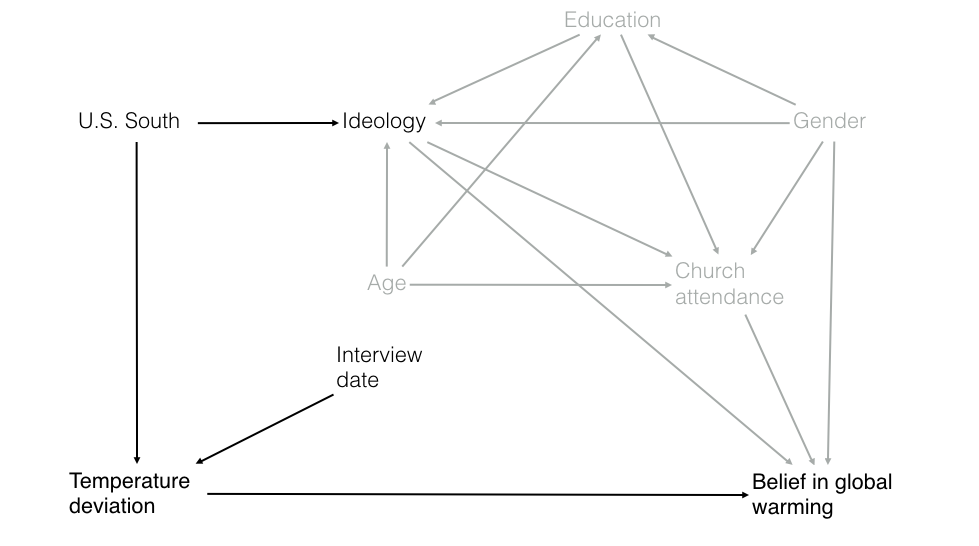
\includegraphics[height=.8\textheight]{../04-figures/03/05-egan&mullin_dag}
    \end{figure}
\end{frame}


\begin{frame}
  \frametitle{Table 1 from Egan and Mullin \citeyear{egan_turning_2012}}
	 \begin{figure} 
    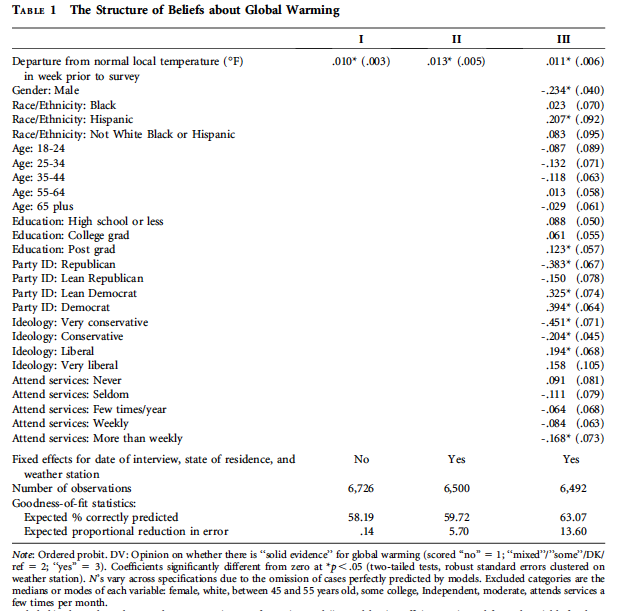
\includegraphics[height=.8\textheight]{../04-figures/03/06-egan&mullin_table1}
    \end{figure}
\end{frame}


\begin{frame}
  \frametitle{A causal effect of post-grad education?}
	 \begin{figure} 
    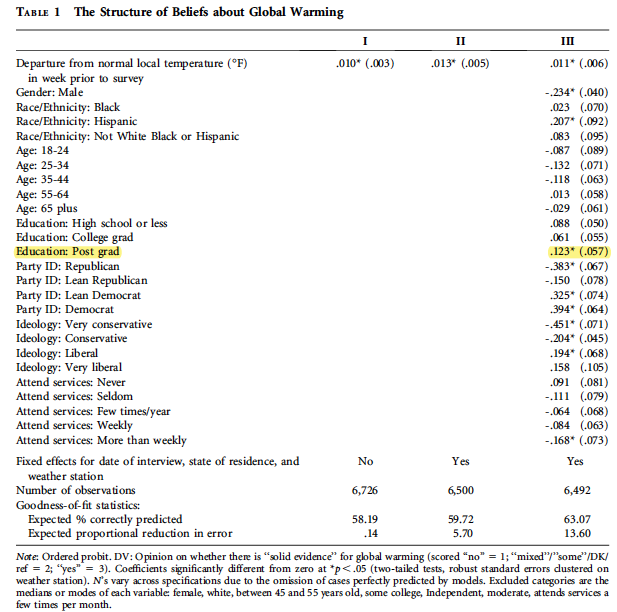
\includegraphics[height=.8\textheight]{../04-figures/03/07-egan&mullin_table1_hl}
    \end{figure}
\end{frame}

\begin{frame}
  \frametitle{A causal effect of post-grad education?}
	 \begin{figure} 
    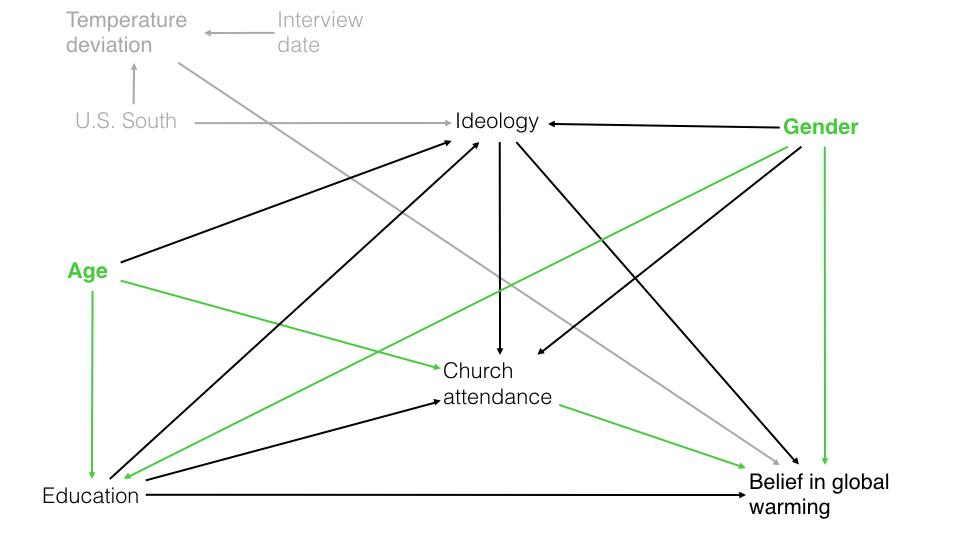
\includegraphics[height=.8\textheight]{../04-figures/03/08-egan&mullin_observables}
    \end{figure}
\end{frame}

\begin{frame}
  \frametitle{A causal effect of post-grad education?}
	 \begin{figure} 
    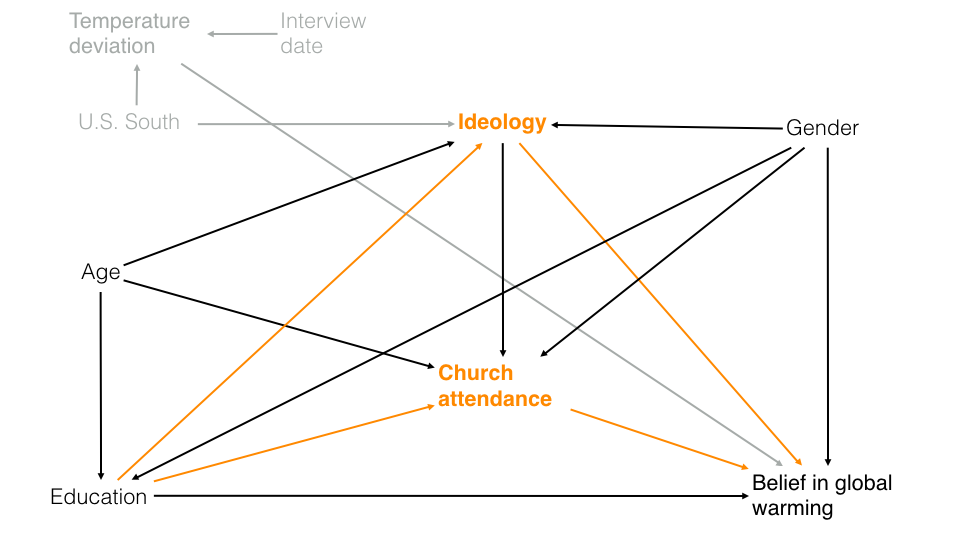
\includegraphics[height=.8\textheight]{../04-figures/03/09-egan&mullin_onpath}
    \end{figure}
\end{frame}


\begin{frame}
  \frametitle{A causal effect of post-grad education?}
	 \begin{figure} 
    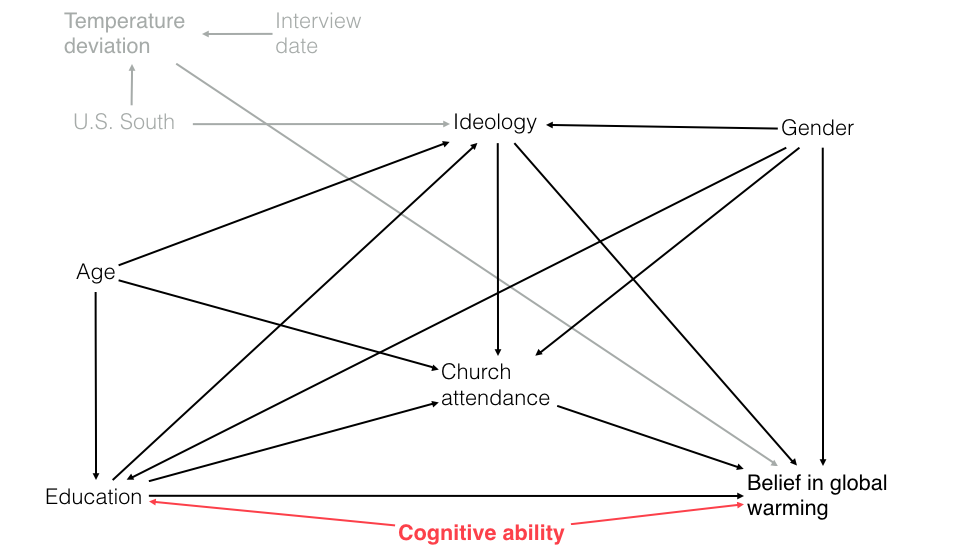
\includegraphics[height=.8\textheight]{../04-figures/03/10-egan&mullin_unobservables}
    \end{figure}
\end{frame}


% END
\begin{frame}
\begin{center}
    \LARGE Thank you for watching, and see you next Monday!
\end{center}
\end{frame}

% REFERENCES %

\begin{frame}
\frametitle{References}
\bibliographystyle{apacite}
\bibliography{../Bibliography}
\vspace{5cm}
\end{frame}

\end{document}
